\documentclass[a4paper,12pt]{article}

\usepackage[utf8x]{inputenc}
\usepackage[T2A]{fontenc}
\usepackage[english, russian]{babel}

% Опционно, требует  apt-get install scalable-cyrfonts.*
% и удаления одной строчки в cyrtimes.sty
% Сточку не удалять!
% \usepackage{cyrtimes}

% Картнки и tikz
\usepackage{graphicx}
\usepackage{tikz}
\usetikzlibrary{snakes,arrows,shapes}


% Некоторая русификация.
\usepackage{misccorr}
\usepackage{indentfirst}
\renewcommand{\labelitemi}{\normalfont\bfseries{--}}

% Увы, поля придётся уменьшить из-за листингов.
\topmargin -1cm
\oddsidemargin -0.5cm
\evensidemargin -0.5cm
\textwidth 17cm
\textheight 24cm

\sloppy

% Оглавление в PDF
\usepackage[
bookmarks=true,
colorlinks=true, linkcolor=black, anchorcolor=black, citecolor=black, menucolor=black,filecolor=black, urlcolor=black,
unicode=true
]{hyperref}

% Для исходного кода в тексте
\newcommand{\Code}[1]{\texttt{#1}}


\title{Отчёт по лабораторной работе \\ <<Система доменных имён>>}
\author{(Фроловского Алексея Вадимовича)}

\begin{document}

\maketitle

\tableofcontents

\section{Настройка системы DNS}

\subsection{Топология сети}

Топология сети и использыемые IP-адреса показаны на рис.~\ref{fig:network}.

\begin{figure}
\centering
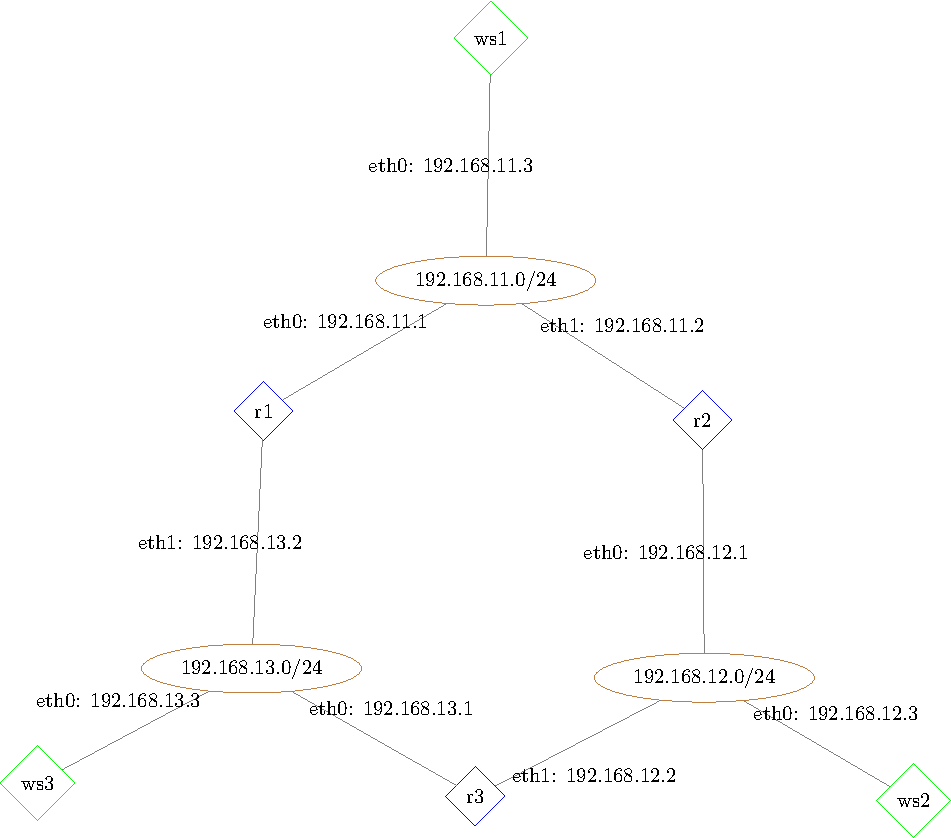
\includegraphics[width=\textwidth]{includes/network_gv.pdf}
\caption{Топология сети}
\label{fig:network}
\end{figure}

\subsection{Структура службы доменных имён}

Структура авторитетных серверов доменных имён показана на рис.~\ref{fig:dns}.

\begin{figure}
\centering
\includegraphics[width=\textwidth]{includes/dns_gv.pdf}
\caption{Структура службы доменных имён}
\label{fig:dns}
\end{figure}

\subsection{Прочие настройки}

Кеширующие DNS-серверы
\begin{itemize}
\item 2.0.5.1;
\item 2.0.6.1;
\item 2.0.7.1
\end{itemize}

Развёрнутые SMTP-серверы и используемые ими кеширующие DNS-серверы.
\begin{itemize}
\item  использует сервер на ... ;
\item ...
\end{itemize}


\section{Проверка настройки службы доменных имён}

\subsection{Проверка настройки записи типа MX для домена paris.france}

\begin{verbatim}
mail1:~# dig @2.0.0.1 paris.france MX

; <<>> DiG 9.5.0-P2 <<>> @2.0.0.1 paris.france MX
; (1 server found)
;; global options:  printcmd
;; Got answer:
;; ->>HEADER<<- opcode: QUERY, status: NOERROR, id: 24158
;; flags: qr rd; QUERY: 1, ANSWER: 0, AUTHORITY: 1, ADDITIONAL: 1
;; WARNING: recursion requested but not available

;; QUESTION SECTION:
;paris.france.			IN	MX

;; AUTHORITY SECTION:
france.			86400	IN	NS	ns1.france.

;; ADDITIONAL SECTION:
ns1.france.		86400	IN	A	2.0.2.1

;; Query time: 27 msec
;; SERVER: 2.0.0.1#53(2.0.0.1)
;; WHEN: Fri Dec 13 13:57:47 2013
;; MSG SIZE  rcvd: 64
\end{verbatim}

\begin{verbatim}
mail1:~# dig @2.0.2.1 paris.france MX

; <<>> DiG 9.5.0-P2 <<>> @2.0.2.1 paris.france MX
; (1 server found)
;; global options:  printcmd
;; Got answer:
;; ->>HEADER<<- opcode: QUERY, status: NOERROR, id: 43246
;; flags: qr aa rd; QUERY: 1, ANSWER: 1, AUTHORITY: 2, ADDITIONAL: 2
;; WARNING: recursion requested but not available

;; QUESTION SECTION:
;paris.france.			IN	MX

;; ANSWER SECTION:
paris.france.		86400	IN	MX	10 mail.paris.france.

;; AUTHORITY SECTION:
paris.france.		86400	IN	NS	ns1.paris.france.
paris.france.		86400	IN	NS	ns1.france.

;; ADDITIONAL SECTION:
mail.paris.france.	86400	IN	A	2.0.7.1
ns1.france.		86400	IN	A	2.0.2.1

;; Query time: 13 msec
;; SERVER: 2.0.2.1#53(2.0.2.1)
;; WHEN: Fri Dec 13 13:58:25 2013
;; MSG SIZE  rcvd: 119
\end{verbatim}

Или
\begin{Verbatim}
mail1:~# dig @2.0.4.1 paris.france MX

; <<>> DiG 9.5.0-P2 <<>> @2.0.4.1 paris.france MX
; (1 server found)
;; global options:  printcmd
;; Got answer:
;; ->>HEADER<<- opcode: QUERY, status: NOERROR, id: 34847
;; flags: qr aa rd; QUERY: 1, ANSWER: 1, AUTHORITY: 2, ADDITIONAL: 1
;; WARNING: recursion requested but not available

;; QUESTION SECTION:
;paris.france.			IN	MX

;; ANSWER SECTION:
paris.france.		86400	IN	MX	10 mail.paris.france.

;; AUTHORITY SECTION:
paris.france.		86400	IN	NS	ns1.france.
paris.france.		86400	IN	NS	ns1.paris.france.

;; ADDITIONAL SECTION:
mail.paris.france.	86400	IN	A	2.0.7.1

;; Query time: 35 msec
;; SERVER: 2.0.4.1#53(2.0.4.1)
;; WHEN: Fri Dec 13 13:59:08 2013
;; MSG SIZE  rcvd: 103
\end{Verbatim}

Опрашиваем кеширующий DNS-сервер.
\begin{Verbatim}
mail1:~# dig @127.0.0.1 paris.france MX

; <<>> DiG 9.5.0-P2 <<>> @127.0.0.1 paris.france MX
; (1 server found)
;; global options:  printcmd
;; Got answer:
;; ->>HEADER<<- opcode: QUERY, status: NOERROR, id: 22360
;; flags: qr rd ra; QUERY: 1, ANSWER: 1, AUTHORITY: 0, ADDITIONAL: 1

;; QUESTION SECTION:
;paris.france.			IN	MX

;; ANSWER SECTION:
paris.france.		85781	IN	MX	10 mail.paris.france.

;; ADDITIONAL SECTION:
mail.paris.france.	85781	IN	A	2.0.7.1

;; Query time: 20 msec
;; SERVER: 127.0.0.1#53(127.0.0.1)
;; WHEN: Fri Dec 13 14:00:17 2013
;; MSG SIZE  rcvd: 67
\end{Verbatim}

\begin{verbatim}
mail1:~# ping mail.paris.france
PING mail.paris.france (2.0.7.1) 56(84) bytes of data.
64 bytes from 2.0.7.1: icmp_seq=1 ttl=64 time=7.92 ms
64 bytes from 2.0.7.1: icmp_seq=2 ttl=64 time=0.716 ms
64 bytes from 2.0.7.1: icmp_seq=3 ttl=64 time=0.638 ms
64 bytes from 2.0.7.1: icmp_seq=4 ttl=64 time=0.634 ms
64 bytes from 2.0.7.1: icmp_seq=5 ttl=64 time=0.452 ms
64 bytes from 2.0.7.1: icmp_seq=6 ttl=64 time=0.547 ms
64 bytes from 2.0.7.1: icmp_seq=7 ttl=64 time=0.557 ms
64 bytes from 2.0.7.1: icmp_seq=8 ttl=64 time=0.270 ms
64 bytes from 2.0.7.1: icmp_seq=9 ttl=64 time=0.563 ms
64 bytes from 2.0.7.1: icmp_seq=10 ttl=64 time=0.853 ms
64 bytes from 2.0.7.1: icmp_seq=11 ttl=64 time=0.271 ms
64 bytes from 2.0.7.1: icmp_seq=12 ttl=64 time=0.633 ms
64 bytes from 2.0.7.1: icmp_seq=13 ttl=64 time=0.693 ms
64 bytes from 2.0.7.1: icmp_seq=14 ttl=64 time=0.662 ms
64 bytes from 2.0.7.1: icmp_seq=15 ttl=64 time=0.641 ms
64 bytes from 2.0.7.1: icmp_seq=16 ttl=64 time=0.850 ms
64 bytes from 2.0.7.1: icmp_seq=17 ttl=64 time=0.694 ms
64 bytes from 2.0.7.1: icmp_seq=18 ttl=64 time=0.400 ms
64 bytes from 2.0.7.1: icmp_seq=19 ttl=64 time=0.408 ms
64 bytes from 2.0.7.1: icmp_seq=20 ttl=64 time=0.746 ms
^C
--- mail.paris.france ping statistics ---
20 packets transmitted, 20 received, 0% packet loss, time 19185ms
rtt min/avg/max/mdev = 0.270/0.957/7.928/1.607 ms
\end{verbatim}

\subsection{Проверка настройки записи типа ... для домена ...}

Повторяем далее.

\section{Проверка работы почтовой системы}

\subsection{Проверка MX-записи для домена ...}

С узла ... отправили письмо на локальный SMTP-сервер для адресата с адресом .....

\begin{verbatim}
Сюда нужно поместить лог работы с SMTP-сервером.
\end{verbatim}

На машине с доменным именем ... появилось доставленное письмо.
\begin{verbatim}
Результат cat /var/mail/...
\end{verbatim}

Таким образом, доменная запись типа MX для домена ... настроена верно.

\subsection{Проверка MX-записи для домена ...}

(повторить для всех SMTP-серверов)

\end{document}
